% Appendix 5: The Cross Product of Two Vectors
% VIC Specialist Mathematics — Units 3–4; QLD Specialist Mathematics — Unit 3
%
% This appendix merges the former §1.4.13 enrichment with additional
% worked examples and applications from the VIC/QLD syllabuses.
\begingroup
\small

\noindent\fbox{%
\begin{minipage}{0.97\textwidth}
\textit{\textbf{Enrichment only.}
The cross product is part of
\textbf{VIC Specialist Mathematics (Units~3--4)} and
\textbf{QLD Specialist Mathematics (Unit~3)}.
It is \textbf{not} prescribed in the current NESA
Mathematics Extension~1 or Extension~2 syllabus, so none of the core
worked methods in Parts~1 and~2 of this booklet depend on it.
It is included here because students may meet it later in university
mathematics, physics, or engineering, and it can help connect familiar
vector ideas to further study.}
\end{minipage}}

\vspace{0.8em}

% ---- Key concepts ----
\noindent\textbf{Key concepts.}

The dot product produces a \emph{scalar}:
\[
  \mathbf{a} \cdot \mathbf{b}
  = |\mathbf{a}|\,|\mathbf{b}|\cos\theta.
\]
The \textbf{cross product} produces a \emph{vector} perpendicular to
both original vectors.

For two vectors in three dimensions,
\[
  \mathbf{a} = (a_1,\, a_2,\, a_3),
  \qquad
  \mathbf{b} = (b_1,\, b_2,\, b_3),
\]
their cross product is defined by
\[
  \boxed{
  \mathbf{a} \times \mathbf{b}
  = \begin{pmatrix}
      a_2 b_3 - a_3 b_2 \\
      a_3 b_1 - a_1 b_3 \\
      a_1 b_2 - a_2 b_1
    \end{pmatrix}}.
\]

\vspace{0.4em}
\noindent\textbf{Determinant mnemonic.}
The same formula can be written using a $3\times 3$ determinant
expansion:
\[
  \mathbf{a} \times \mathbf{b}
  = \begin{vmatrix}
      \mathbf{i} & \mathbf{j} & \mathbf{k} \\
      a_1 & a_2 & a_3 \\
      b_1 & b_2 & b_3
    \end{vmatrix}
  = \begin{vmatrix} a_2 & a_3 \\ b_2 & b_3 \end{vmatrix}\mathbf{i}
  - \begin{vmatrix} a_1 & a_3 \\ b_1 & b_3 \end{vmatrix}\mathbf{j}
  + \begin{vmatrix} a_1 & a_2 \\ b_1 & b_2 \end{vmatrix}\mathbf{k}.
\]

\noindent\textbf{Understanding the matrix notation.}
Because matrices and determinants are not taught in the NSW HSC
syllabus, this notation is used here purely as a practical calculation
mnemonic (recipe):
\begin{itemize}[leftmargin=*,itemsep=1pt,topsep=2pt]
  \item \textbf{$2\times 2$ Determinant (Criss-Cross):}
    $\begin{vmatrix} p & q \\ r & s \end{vmatrix} = ps - qr$
    (main diagonal minus off-diagonal).
  \item \textbf{Top-Row Expansion:} For each unit vector
    ($\mathbf{i}$, $\mathbf{j}$, $\mathbf{k}$), delete its row and
    column; the remaining four entries form a $2\times 2$
    sub-determinant.
  \item \textbf{Alternating Signs ($+, -, +$):} Notice the
    \textbf{minus sign} on the middle $\mathbf{j}$ component:
    $-(a_1 b_3 - a_3 b_1)\mathbf{j}$, which is the most frequent
    source of errors.
\end{itemize}

\vspace{0.4em}
\noindent\textbf{Magnitude and direction.}
\[
  \boxed{
  |\mathbf{a} \times \mathbf{b}|
  = |\mathbf{a}|\,|\mathbf{b}|\sin\theta
  }
\]
where $0 \le \theta \le \pi$.
The direction follows the \textbf{right-hand rule}.
In particular,
\[
  \mathbf{a} \times \mathbf{b}
  = -(\mathbf{b} \times \mathbf{a}).
\]

The cross product has an elegant geometric interpretation: its
magnitude is the area of the parallelogram formed by the two vectors.

\vspace{0.4em}
\noindent\textbf{Properties.}
\begin{itemize}[leftmargin=*,itemsep=1pt,topsep=2pt]
  \item $\mathbf{a} \times \mathbf{b}$ is perpendicular to both
        $\mathbf{a}$ and $\mathbf{b}$.
  \item $|\mathbf{a} \times \mathbf{b}|
        = |\mathbf{a}|\,|\mathbf{b}|\sin\theta$
        (area of parallelogram).
  \item $\mathbf{a} \times \mathbf{b}
        = -\mathbf{b} \times \mathbf{a}$ (anticommutative).
  \item Two vectors have zero cross product precisely when they are
        parallel, including the case where one is the zero vector.
\end{itemize}

% ---- Diagrams ----
\begin{center}
\tdplotsetmaincoords{70}{120}
\begin{tikzpicture}[tdplot_main_coords,scale=1.1]
  % Origin
  \coordinate (O) at (0,0,0);

  % Vector a
  \coordinate (A) at (3,1,0);
  \draw[->,very thick,blue] (O) -- (A) node[midway,below] {$\mathbf{a}$};

  % Vector b
  \coordinate (B) at (1,3,0.5);
  \draw[->,very thick,red] (O) -- (B) node[midway,left] {$\mathbf{b}$};

  % Cross product vector (perpendicular to both a and b)
  \coordinate (C) at (0,0,3);
  \draw[->,ultra thick,green!60!black] (O) -- (C)
    node[midway,right] {$\mathbf{a}\times\mathbf{b}$};

  % Parallelogram formed by a and b
  \coordinate (P) at (4,4,0.5);
  \draw[dashed,orange,thick] (A) -- (P);
  \draw[dashed,orange,thick] (B) -- (P);
  \fill[blue!20,opacity=0.4] (O) -- (A) -- (P) -- (B) -- cycle;

  % Right angle indicators
  \draw[thick,green!60!black] (0.3,0.1,0) -- (0.3,0.1,0.3) -- (0,0.1,0.3);
  \draw[thick,green!60!black] (0.1,0.3,0) -- (0.1,0.3,0.3) -- (0.1,0,0.3);

  % Angle theta
  \tdplotsetrotatedcoords{0}{0}{0}
  \tdplotdrawarc[thick,tdplot_rotated_coords]{(O)}{0.6}{18}{70}%
    {anchor=south west}{$\theta$}

  % Origin point
  \node[circle,fill=black,inner sep=2pt] at (O) {};

  % Axes
  \draw[gray,->] (O) -- (4,0,0) node[anchor=north east]{$x$};
  \draw[gray,->] (O) -- (0,4.5,0) node[anchor=north west]{$y$};
  \draw[gray,->] (O) -- (0,0,3.5) node[anchor=south]{$z$};
\end{tikzpicture}
\hspace{0.5cm}
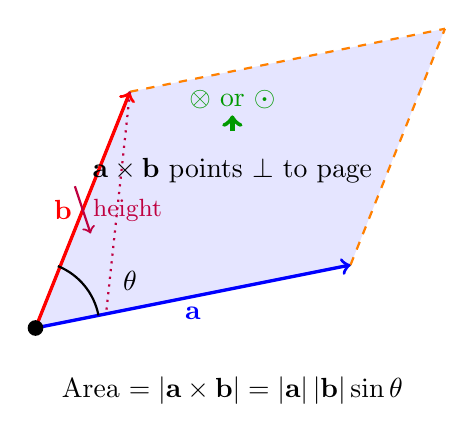
\begin{tikzpicture}[scale=1.0]
  % 2D view showing parallelogram area
  \coordinate (O) at (0,0);
  \coordinate (A) at (4,0.8);
  \coordinate (B) at (1.2,3);
  \coordinate (P) at (5.2,3.8);

  % Parallelogram
  \fill[blue!20,opacity=0.5] (O) -- (A) -- (P) -- (B) -- cycle;
  \draw[thick] (O) -- (A);
  \draw[thick] (O) -- (B);
  \draw[dashed,orange,thick] (A) -- (P);
  \draw[dashed,orange,thick] (B) -- (P);

  % Vectors
  \draw[->,very thick,blue] (O) -- (A) node[midway,below] {$\mathbf{a}$};
  \draw[->,very thick,red] (O) -- (B) node[midway,left] {$\mathbf{b}$};

  % Angle
  \draw[thick] (0.8,0.16) arc (11:68:0.85);
  \node at (1.2,0.6) {$\theta$};

  % Height line
  \coordinate (H) at (0.896,0.179);
  \draw[dotted,thick,purple] (B) -- (H);
  \draw[->,thick,purple] (0.5,1.8) -- (0.7,1.2)
    node[midway,right] {\small height};

  % Origin point
  \node[circle,fill=black,inner sep=2pt] at (O) {};

  % Area label
  \node[anchor=north] at (2.5,-0.5)
    {Area $= |\mathbf{a}\times\mathbf{b}|
           = |\mathbf{a}|\,|\mathbf{b}|\sin\theta$};

  % Cross product direction indicator
  \node at (2.5,2) {$\mathbf{a}\times\mathbf{b}$ points $\perp$ to page};
  \draw[->,ultra thick,green!60!black] (2.5,2.5) -- (2.5,2.7);
  \node[green!60!black] at (2.5,2.9) {$\otimes$ or $\odot$};
\end{tikzpicture}
\end{center}

\vspace{0.5em}
\noindent\textit{Left:} The cross product
$\mathbf{a}\times\mathbf{b}$ (green) is perpendicular to both
$\mathbf{a}$ (blue) and $\mathbf{b}$ (red), using the right-hand
rule for direction.
\textit{Right:} The magnitude $|\mathbf{a}\times\mathbf{b}|$ equals
the area of the parallelogram formed by $\mathbf{a}$ and $\mathbf{b}$.

% ---- Worked Example 1: Triangle area ----
\vspace{0.8em}
\noindent\textbf{Worked example~1 --- Cross product and triangle area.}

\noindent Given
\[
  \mathbf{a} = (1,0,1),
  \qquad
  \mathbf{b} = (0,2,0),
\]
find: (a) $\mathbf{a}\times\mathbf{b}$; \quad
      (b) the area of the triangle formed by the two vectors.

\vspace{0.3em}
\noindent\textit{Solution.}
Using the component formula,
\[
  \mathbf{a} \times \mathbf{b}
  = \bigl(0\cdot 0 - 1\cdot 2,\;
         1\cdot 0 - 1\cdot 0,\;
         1\cdot 2 - 0\cdot 0\bigr)
  = \boxed{(-2,\, 0,\, 2)}.
\]
Its magnitude is
\[
  |\mathbf{a} \times \mathbf{b}|
  = \sqrt{(-2)^{2} + 0^{2} + 2^{2}}
  = 2\sqrt{2}.
\]
The triangle has half the area of the parallelogram:
\[
  \boxed{\text{Area of triangle} = \sqrt{2}}.
\]

\noindent\textit{Verification of perpendicularity.}
\[
  (\mathbf{a} \times \mathbf{b}) \cdot \mathbf{a}
  = (-2)(1) + 0(0) + 2(1) = 0, \qquad
  (\mathbf{a} \times \mathbf{b}) \cdot \mathbf{b}
  = (-2)(0) + 0(2) + 2(0) = 0.
\]
Thus the cross product is perpendicular to both original vectors.
$\checkmark$

% ---- Worked Example 2: Point-to-line distance ----
\vspace{0.8em}
\noindent\textbf{Worked example~2 --- Distance from point to line.}

\noindent\textit{Problem.}
Find the distance from point $P(1, 2, 0)$ to the line
$\mathbf{r}
= \begin{pmatrix}1\\0\\1\end{pmatrix}
+ \lambda\begin{pmatrix}0\\1\\1\end{pmatrix}$.

\vspace{0.3em}
\noindent\textit{Solution using Cross Product.}
Let $A(1,0,1)$ be a point on the line and
$\mathbf{d} = \begin{pmatrix}0\\1\\1\end{pmatrix}$
be the direction vector.
The vector from $A$ to $P$ is
$\overrightarrow{AP} = \begin{pmatrix}0\\2\\-1\end{pmatrix}$.

Using the cross product:
\[
  \overrightarrow{AP} \times \mathbf{d}
  = \begin{vmatrix}
      \mathbf{i} & \mathbf{j} & \mathbf{k} \\
      0 & 2 & -1 \\
      0 & 1 & 1
    \end{vmatrix}
  = \begin{vmatrix} 2 & -1 \\ 1 & 1 \end{vmatrix}\mathbf{i}
  - \begin{vmatrix} 0 & -1 \\ 0 & 1 \end{vmatrix}\mathbf{j}
  + \begin{vmatrix} 0 & 2 \\ 0 & 1 \end{vmatrix}\mathbf{k}
  = 3\mathbf{i} - 0\mathbf{j} + 0\mathbf{k}
  = \begin{pmatrix}3\\0\\0\end{pmatrix}.
\]

Distance:
$d = \dfrac{|\overrightarrow{AP} \times \mathbf{d}|}{|\mathbf{d}|}
   = \dfrac{3}{\sqrt{2}}
   = \dfrac{3\sqrt{2}}{2}$ units.

\vspace{0.3em}
\noindent\textit{Comparison with the syllabus method.}
The in-syllabus method uses projection.
The component of $\overrightarrow{AP}$ perpendicular to the line is
found by:
\[
  \overrightarrow{AP}_{\perp}
  = \overrightarrow{AP}
  - \frac{\overrightarrow{AP} \cdot \mathbf{d}}
         {\mathbf{d} \cdot \mathbf{d}}\,\mathbf{d}.
\]
Then $d = |\overrightarrow{AP}_{\perp}|$.
Both methods yield the same result; for HSC purposes, the projection
method is the syllabus-aligned approach to remember.

% ---- Worked Example 3: Flattening 3D to 2D ----
\vspace{0.8em}
\noindent\textbf{Worked example~3 --- Flattening 3D to 2D: Triangle Area on an Ellipse.}

\noindent\textit{Problem.}
Let $P(a\cos\theta,\, b\sin\theta)$ and $Q(a\cos\phi,\, b\sin\phi)$ be two points on the ellipse $\frac{x^2}{a^2} + \frac{y^2}{b^2} = 1$, where $a, b > 0$. Find the area of triangle $OPQ$, where $O$ is the origin $(0,0)$.

\vspace{0.3em}
\noindent\textit{Solution using the Cross Product (The ``Two-Line'' Shortcut).}
Embed the two-dimensional position vectors into three-dimensional space by setting the $z$-coordinate to zero:
\[
  \mathbf{p} = \begin{pmatrix} a\cos\theta \\ b\sin\theta \\ 0 \end{pmatrix},
  \qquad
  \mathbf{q} = \begin{pmatrix} a\cos\phi \\ b\sin\phi \\ 0 \end{pmatrix}.
\]
Their cross product points strictly perpendicular to the $xy$-plane along $\mathbf{k}$:
\begin{align*}
  \mathbf{p} \times \mathbf{q}
  &= \begin{vmatrix}
       \mathbf{i} & \mathbf{j} & \mathbf{k} \\
       a\cos\theta & b\sin\theta & 0 \\
       a\cos\phi & b\sin\phi & 0
     \end{vmatrix}
  = 0\mathbf{i} - 0\mathbf{j} + \bigl(ab\cos\theta\sin\phi - ab\sin\theta\cos\phi\bigr)\mathbf{k} \\
  &= ab\sin(\phi - \theta)\,\mathbf{k}.
\end{align*}
The area of the triangle is half the area of the parallelogram formed by $\mathbf{p}$ and $\mathbf{q}$:
\[
  \boxed{\text{Area}(\triangle OPQ) = \frac{1}{2}|\mathbf{p} \times \mathbf{q}| = \frac{1}{2}ab|\sin(\phi - \theta)|}.
\]

\vspace{0.3em}
\noindent\textit{The Historical 4U HSC Pain Point.}
In the pre-2020 NSW HSC Extension~2 (4~Unit) syllabus, conic sections were examined extensively without vector cross products or matrices. Under the standard syllabus method, students had to:
\begin{enumerate}[leftmargin=*,itemsep=1pt]
  \item Apply the distance formula to find the base length $PQ = \sqrt{a^2(\cos\phi - \cos\theta)^2 + b^2(\sin\phi - \sin\theta)^2}$.
  \item Determine the Cartesian equation of the chord $PQ$: $(b\cos\tfrac{\theta+\phi}{2})x + (a\sin\tfrac{\theta+\phi}{2})y = ab\cos\tfrac{\phi-\theta}{2}$.
  \item Apply the perpendicular distance formula $h = \frac{|Ax_0 + By_0 + C|}{\sqrt{A^2 + B^2}}$ from $O(0,0)$ to the chord.
  \item Calculate $\text{Area} = \frac{1}{2} \times \text{base} \times \text{height}$, expanding pages of nested square roots and trig identities to obtain cancellations.
\end{enumerate}
With the cross product, this entire algebraic marathon collapses into two elementary lines!

\vspace{0.3em}
\noindent\textit{Connection to Matrices.}
Notice that the $\mathbf{k}$-component of $\mathbf{p}\times\mathbf{q}$ is identically the $2\times 2$ matrix determinant $\det \begin{pmatrix} a\cos\theta & b\sin\theta \\ a\cos\phi & b\sin\phi \end{pmatrix}$. For full coverage of coordinate determinants and the general $3\times 3$ area formula $\frac{1}{2}\left|\det \begin{pmatrix} x_1 & y_1 & 1 \\ x_2 & y_2 & 1 \\ x_3 & y_3 & 1 \end{pmatrix}\right|$, see our companion booklet \emph{Matrix Practice: NSW Extension Enrichment \& QLD Specialist Mathematics}.

% ---- Key takeaways ----
\vspace{0.8em}
\noindent\textbf{Key takeaways.}
\begin{itemize}[leftmargin=*,itemsep=2pt]
  \item The dot product measures how much two vectors point in the
        same direction; the cross product gives a perpendicular
        direction and an area.
  \item In 2D plane geometry, embedding vectors into 3D with $z=0$ turns
        triangle and polygon area calculations into a one-step cross
        product, bypassing tedious coordinate geometry formulas.
  \item Two vectors have zero cross product precisely when they are
        parallel, including the case where one is the zero vector.
  \item The order matters:
        $\mathbf{a}\times\mathbf{b} \ne \mathbf{b}\times\mathbf{a}$
        in general.
\end{itemize}

\vspace{0.4em}
\noindent\textit{Beyond school --- University connection.}
The cross product appears in rotational mechanics, electromagnetism
and computer graphics. For example, the torque produced by a force is
\[
  \boldsymbol{\tau} = \mathbf{r} \times \mathbf{F},
\]
where $\mathbf{r}$ is a position vector and $\mathbf{F}$ is the
applied force.

\endgroup
